\section{ERFINV Inverse Error Function}

\subsection{Usage}

Computes the inverse error function for each element of x.  The \verb|erf|
function takes only a single argument
\begin{verbatim}
  y = erfinv(x)
\end{verbatim}
where \verb|x| is either a \verb|float| or \verb|double| array.  The output
vector \verb|y| is the same size (and type) as \verb|x|. For values outside the interval [-1, 1] function returns NaN.
\subsection{Example}

Here is a plot of the erf function over the range \verb|[-.9,.9]|.
\begin{verbatim}
--> x = linspace(-.9,.9,100);
--> y = erfinv(x);
--> plot(x,y); xlabel('x'); ylabel('erfinv(x)');
\end{verbatim}
which results in the following plot.


\centerline{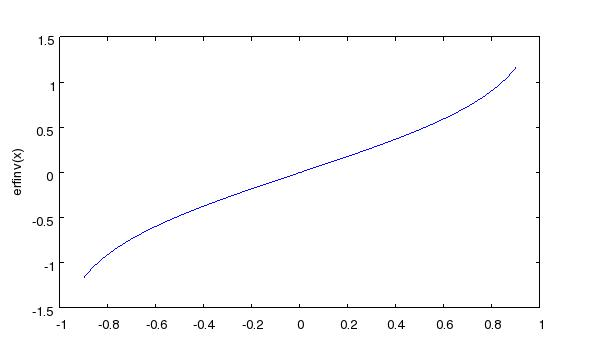
\includegraphics[width=8cm]{erfinv1}}

